\section{Flexible Activation Function for NNs}
We have already seen in \autoref{tab:fitpdf} that the \sindist{} can take the shape of a Logistic (0,1) distribution with great accuracy. Given the closeness of its CDF to the sigmoid activation function, and the additional ability to take on other shapes as well, we aim to construct a neural network endowed with a flexible skewness-kurtosis activation function. This learnable-parameter NN will require deriving custom back-propagation equations for parameter estimation. We will also assess the additional cost of training such a neural network and the benefits associated with the same.

\cite{buzsaki2014log} highlights the presence of skewed activation functions in the brain itself. That asymmetric activation functions perform well has been studied in \cite{junior2025skew}. \cite{kuccukali2026sslu} have also constructed several new skewed activation functions.

\subsection{Varieties of activation functions}
Demarcate the \textbf{bottom (B) and upper (U) ``arms''} of an activation function (equivalently its left and right arms respectively, since an activation function is always non-decreasing) as the 2 parts of the activation function's curve close to horizontal but not exactly flat. We choose the portions of the curve contained in the Y-axis windows $(0,0.1]$ and $[0.9, 1)$ for the purpose of demarcating the arms, although a more objective method of demarcation may involve the inflexion points. Call the segment joining the 2 arms a \textbf{ramp}.

\begin{figure}[h!]
	\centering
	\begin{subfigure}{0.3\linewidth}
		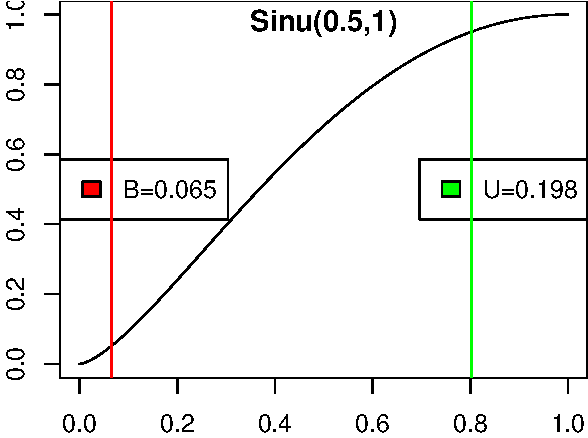
\includegraphics[width=\linewidth]{fig/4.9-CDF (2)}
	\end{subfigure}
	\begin{subfigure}{0.3\linewidth}
		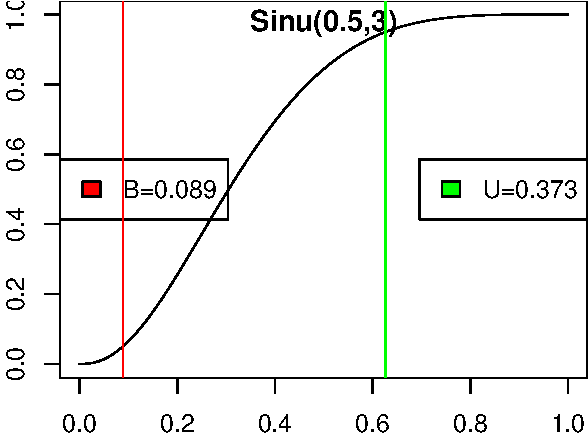
\includegraphics[width=\linewidth]{fig/4.9-CDF (3)}
	\end{subfigure}
	\begin{subfigure}{0.3\linewidth}
		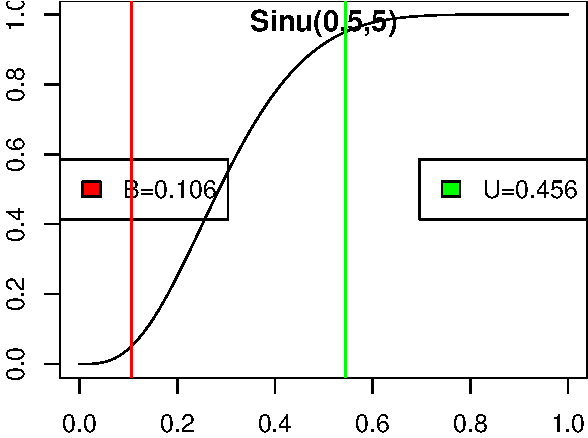
\includegraphics[width=\linewidth]{fig/4.9-CDF (4)}
	\end{subfigure}
	\begin{subfigure}{0.3\linewidth}
		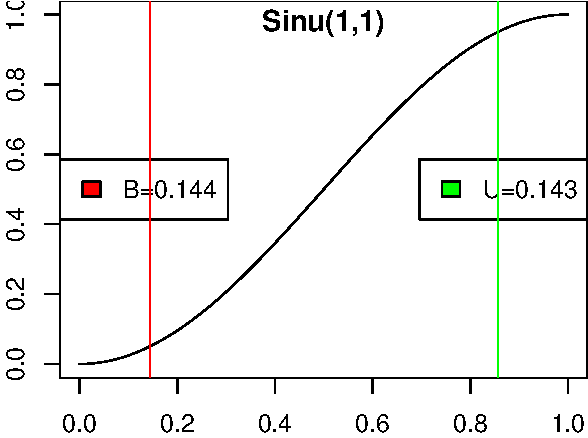
\includegraphics[width=\linewidth]{fig/4.9-CDF (5)}
	\end{subfigure}
	\begin{subfigure}{0.3\linewidth}
		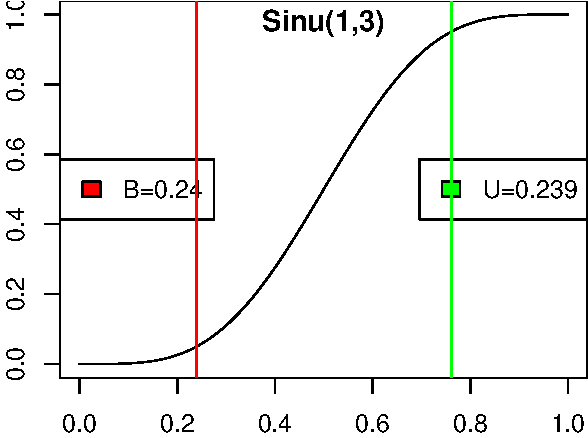
\includegraphics[width=\linewidth]{fig/4.9-CDF (6)}
	\end{subfigure}
	\begin{subfigure}{0.3\linewidth}
		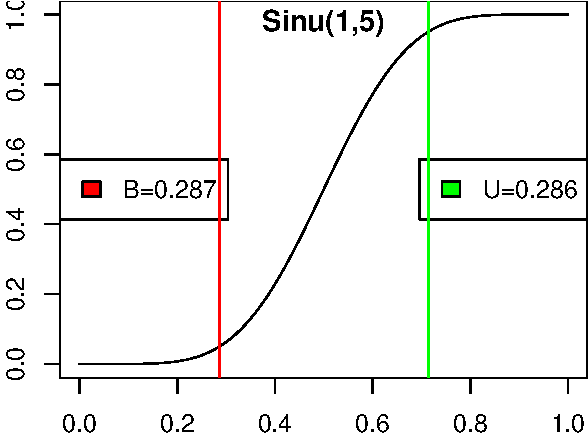
\includegraphics[width=\linewidth]{fig/4.9-CDF (7)}
	\end{subfigure}
	\begin{subfigure}{0.3\linewidth}
		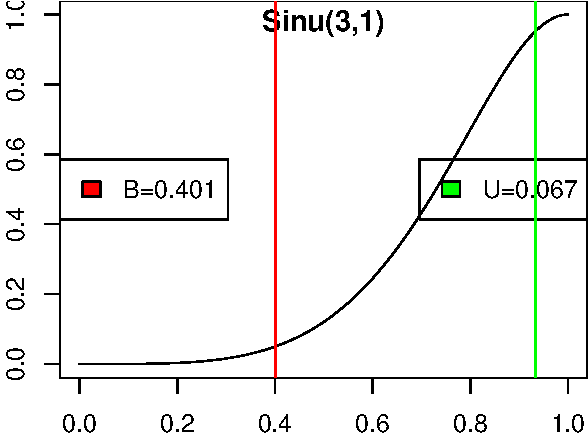
\includegraphics[width=\linewidth]{fig/4.9-CDF (8)}
	\end{subfigure}
	\begin{subfigure}{0.3\linewidth}
		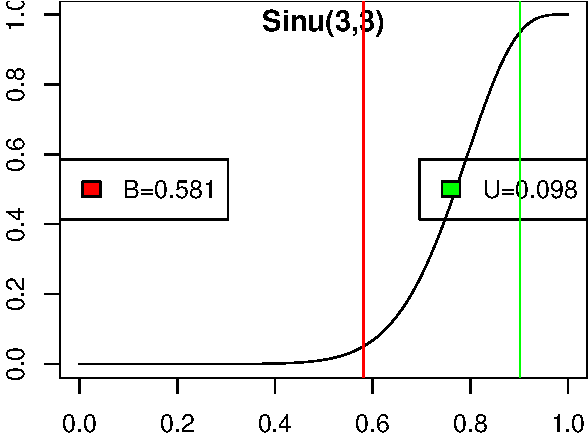
\includegraphics[width=\linewidth]{fig/4.9-CDF (9)}
	\end{subfigure}
		\begin{subfigure}{0.3\linewidth}
		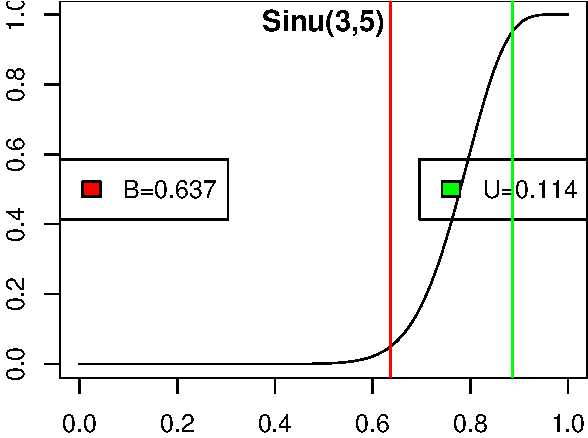
\includegraphics[width=\linewidth]{fig/4.9-CDF (10)}
	\end{subfigure}
	\caption{Different \sindist s as activation functions. U and B are the lengths of the upper and bottom arms respectively. Each upper arm starts at the green line and goes upto $x{=}1$ and each bottom arm starts at $x{=}0$ and goes upto the red line. The segment in between the 2 lines is the ``ramp''.}
	\label{fig:nn-cdfs}
\end{figure}

\begin{table}[h!]
	\begin{tabularx}{\linewidth}{|c|X|X|X|}
		\hline
		& $s=0.5$ & $s=1$ & $s=3$ \\
		\hline
		$k=1$
		& Early onset \newline Early saturation
		& Moderate onset \newline Early saturation
		& Delayed onset \newline Delayed saturation \\
		\hline
		$k=3$
		& Early onset \newline Moderate saturation
		& Moderate onset \newline Moderate saturation
		& Delayed onset \newline Moderate saturation \\
		\hline
		$k=5$
		& Early onset \newline Delayed saturation
		& Moderate onset \newline Moderate saturation
		& Delayed onset \newline Moderate saturation \\
		\hline
	\end{tabularx}
	\caption{A heuristic interpretation of the activation behaviour of various Sinu activation functions based on the lower-arm ($B$) and upper-arm ($U$) lengths.}
	\label{tab:activationfn_vars}
\end{table}

A note about the nomenclature is as follows: Smaller values of $B$ indicate that the activation function leaves the neighbourhood of $0$ quickly, corresponding to an \emph{early onset}, whereas larger values of $B$ imply a more \emph{delayed onset}. Similarly, since $U$ denotes the length of the upper arm before attaining the saturated state $1$, smaller values of $U$ indicate that the function reaches saturation only near the end of the domain, corresponding to \emph{delayed saturation}. Conversely, larger values of $U$ imply an \emph{early saturation}. Intermediate values are heuristically termed \emph{moderate}.

Note how an $s$ far-away from 1 (close to 0 XOR $\infty$) causes imbalanced arms. Again, a larger $k$ causes larger arms and a steeper ramp thereby.


\subsection{Methodology and Results}
We chose one of the most elementary machine learning routines -- classification of the MNIST dataset -- using a relatively simple feed-forward neural network architecture with 2 hidden layers of sizes 256 and 128 respectively. The input layer gets a $28 \times 28$ matrix of black-and-white pixels of handwritten digits, i.e. upon normalization, a vector from $[0,1]^{28 \times 28}$. Corresponding to each digit is present a label: the true digit value of the inscription. The model trains on a training subset of the data

To ensure fair comparison of the effectiveness of the aforementioned 9 different standard \sindist s as activation functions, we replaced them in the aforementioned model each time as the candidate activation function, keeping all other model properties unchanged. Also for reference, we took the (a) vanilla sigmoid, (b) GELU, and (c) SiLU/Swish functions, using them one-by-one as activation functions in the otherwise intact NN architecture. More details about the GELU and SiLU activation functions are available in \autoref{subsec:GELUSilU}.

\begin{figure}[h!]
	\centering
	
	\begin{subfigure}{0.48\linewidth}
		\centering
		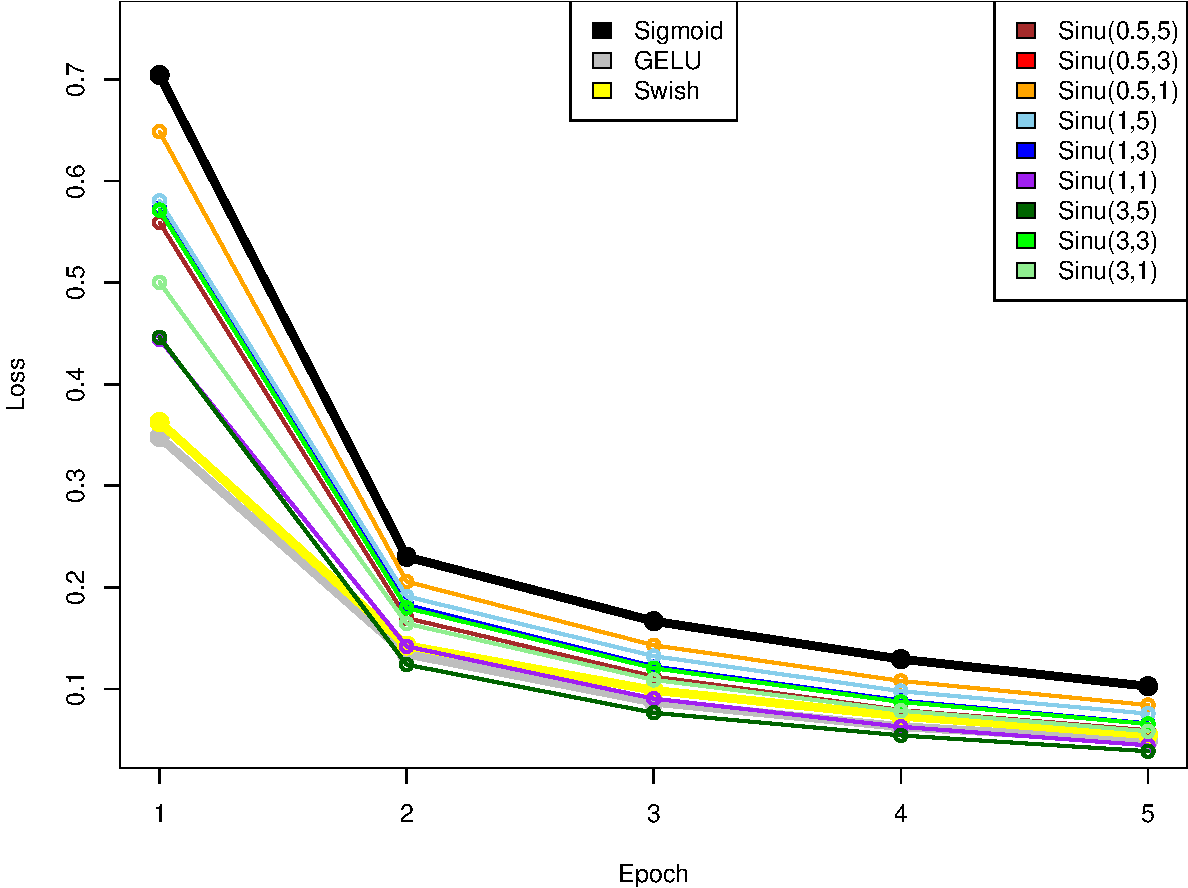
\includegraphics[width=\linewidth]{fig/4.9-NN-Loss}
		\caption{Loss of different models}
		\label{fig:nn-loss}
	\end{subfigure}
	\hfill
	\begin{subfigure}{0.48\linewidth}
		\centering
		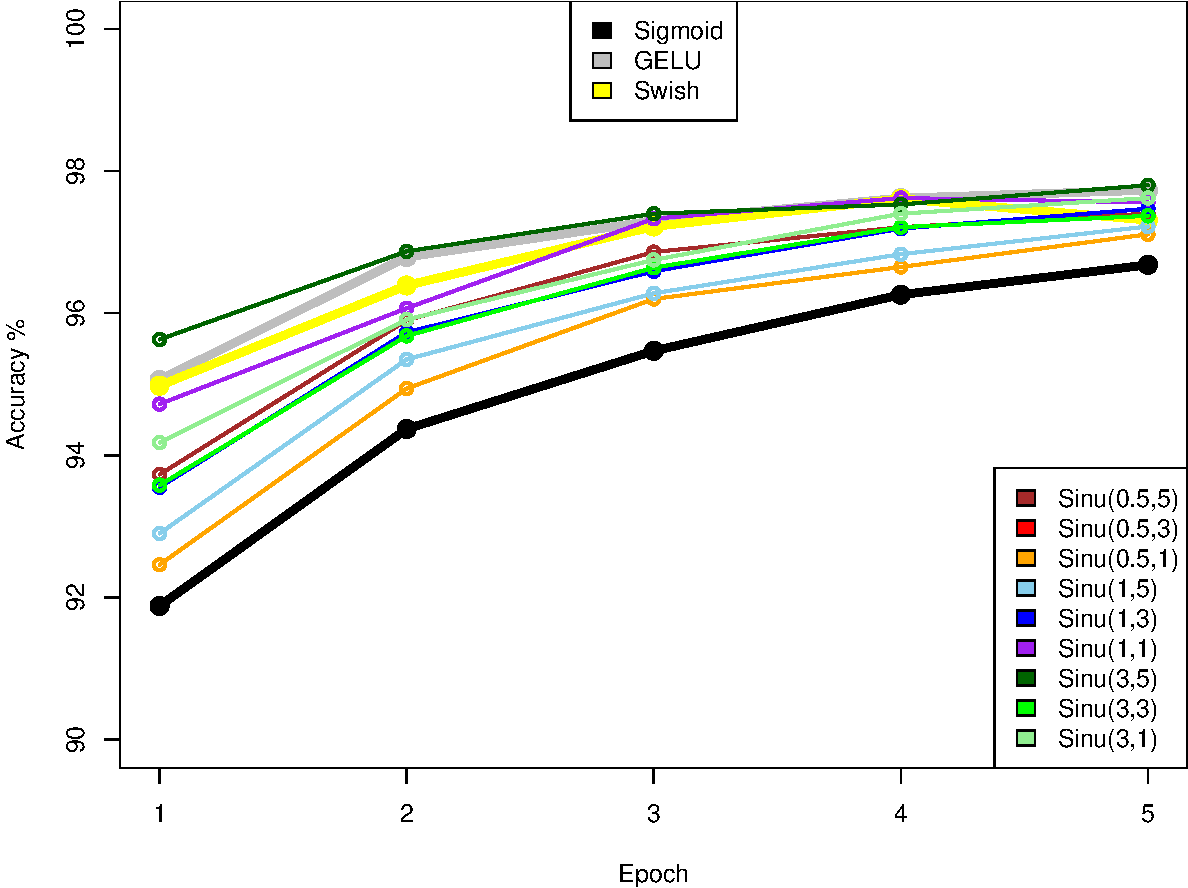
\includegraphics[width=\linewidth]{fig/4.9-NN-Acc}
		\caption{Accuracy of different models}
		\label{fig:nn-acc}
	\end{subfigure}
	
	\caption{Performance of different neural network models over 5 epochs of training over the MNIST dataset.}
	\label{fig:nn-performance}
	
\end{figure}

It can be safely said that all activation functions give a generally usable NN model on this particular dataset. The differences are marginal, all within a quite high accuracy / low loss window.

With respect to the control/reference activation functions, we first observe that the Sigmoid activation NN model underperforms in accuracy and undergoes a slower optimization of the loss function than all its competitors. On the other hand, GELU, an activation function frequently used in transformer based NNs, performs better than most of its competitors. Swish is the industry standard for classification tasks: hence it is no wonder that it maintains top-of-the-line performance.

Coming to the \sindist activation function models, the results are varied. The left skewed platykurtic $\Sinu(0.5,1)$ underperforms with the largest loss and the least accuracy amongst its peers by the end of all 5 epochs. The symmetric $\Sinu(1,5)$ and $\Sinu(1,3)$ fare only slightly better. However, most interestingly, the right skewed and leptokurtic $\Sinu(3,5)$ model almost consistently outperforms even the industry standard Swish model in both and accuracy metrics over 4 out of 5 epochs.

\subsection{Discussion and considerations}
An important insight this approach provides us is that \textbf{datasets have their own optimal activation functions}. Whether different datasets share the same optimal activation function, and what factors influence optimality, are questions for further investigation. However, a strong case is to be made for learnable-parameter NNs based upon a flexible, parametric family of activation functions. This setup will allow the data to refine the models' flexible activation function freely as per its own optimality requirements.

During computational experimentation, we found that a $\Sinu(s=5, k=8)$ model performed very poorly, with a reported loss of 2.3013 and a test accuracy of 11.35\% remaining constant over all 5 epochs. It is suspected that a high skewness and high kurtosis produced a steep ramp at the right end, which was virtually inapproximable by our chosen grid approximation and caching methods. Hence the prediction offered by this model was garbage.